% !TeX root = ../install-latex-guide-zh-cn.tex

\chapter*{前言}

以``啸行''名义加入 QQ 群 91940767、478023327、640633524 和 200392395 后,
经常有群友咨询如何安装 \LaTeX.
实际上,
用户安装的是 \LaTeX{} 的\textbf{发行版}和相关的\textbf{编辑器}.
本手册将介绍在\textbf{不存在其他 \LaTeX{} 发行版 (如 C\TeX{} 套装) 的前提下},
在 Windows 11、Ubuntu 22.04 和 macOS 系统中安装
\TeX{}~Live (macOS 中介绍 Mac\TeX)、升级宏包、编译简易文档等相关操作,
并多以介绍命令行操作为主.
有关 MiK\TeX{} 的安装,
可以参考 \href{https://camusecao.top/2021-06-16/MiKTeX/}{MiK\TeX{} 的基本使用}.

本手册还将简要介绍几款常见编辑器的使用方法,
其他编辑器如 \href{https://code.visualstudio.com/}{VS Code},
\href{https://www.vim.org/}{Vim},
用户可自行了解它们的使用方法.
鉴于 WSL 较为特殊,
本手册提供了一份 VS Code 配合
\href{https://marketplace.visualstudio.com/items?itemName=James-Yu.latex-workshop}{LaTeX Workshop}
的自用配置单,
仅供参考.

除在本地安装 \LaTeX{} 发行版和编辑器之外,
本手册还额外补充两款在线的 \LaTeX 平台,
即 \href{http://www.overleaf.com}{Overleaf} 和 \href{https://www.texpage.com/}{TeXPage} 的相关内容.

本手册所涉及到的代码需结合上下文说明, 不能简单地复制粘贴. 红色文字都是可点的超链接, 可直接跳转.
\menu{菜单} 表示软件菜单. \keys{k} 表示键盘按键.
建议用户阅读 \href{https://tug.org/texlive/doc/texlive-zh-cn/texlive-zh-cn.pdf}{texlive-zh-cn}
和 \href{http://mirrors.ctan.org/info/lshort/chinese/lshort-zh-cn.pdf}{lshort-zh-cn}
以更全面地了解基础内容.

必须声明的是,
即便你已经通读本手册和上面提到的两本书,
有很大概率还会碰到很多问题.
这时我希望用户可以按照正确方式提问,
例如提供\textbf{最小工作示例},
并在论坛上面留下你的问题和相应解答以方便后来者.

本手册大部分内容是个人过去一段时间的使用总结, 其中难免有不甚合理或晦涩难懂的部分. 
若用户在阅读本手册的过程中有任何意见和建议,
请发\href{mailto:ranwang.osbert@outlook.com}{邮件}或在
\href{https://github.com/OsbertWang/install-latex-guide-zh-cn/}{GitHub} 中提 issue.
本手册另在\href{https://gitee.com/OsbertWang/install-latex-guide-zh-cn}{码云}%
有备份,
并于 2020 年 7 月提交至 CTAN.


本手册发布后,
\href{https://github.com/EthanDeng}{Dongsheng Deng},
\href{https://github.com/muzimuzhi}{muzimuzhi},
\href{https://github.com/stone-zeng}{Xiangdong Zeng},
\href{https://github.com/tauyoungsama}{tauyoung},
\href{https://github.com/myhsia}{myhsia},
对本手册提出了很好的建议, 并提供了帮助,
其中, 有关 macOS 的内容最初由 Xiangdong Zeng 草拟完成,
而后 Dongsheng Deng, tauyoung 进行了补充,
最近一次更新则由 myhsia 提供.
在此一并感谢.

本手册自 2024 年 4 月开通捐赠渠道.
如果你认为本手册曾经帮助过你,
并且你还愿意继续支持本手册,
本着自愿原则,
你可以扫描以下二维码为本手册捐赠固定金额.
需要说明的是,
捐赠行为不会影响本手册的更新.
衷心感谢你的支持.

\begin{center}
    \begin{tikzpicture}
        \node{\qrcode[height=2cm]{https://qr.alipay.com/fkx19739ugrexpytkwirbe5}};
        \node[rectangle,rounded corners,fill=white]{\faAlipay};
    \end{tikzpicture}
    \begin{tikzpicture}
        \node{\qrcode[height=2cm]{wxp://f2f1ngYJgHLcAYkvo8VUlpSbF5_J5KiktdpOGmnA0ienTGgAgR2x20yWxEjzHWmIZfcT}};
        \node[rectangle,rounded corners,fill=white]{\faWeixin};
      \end{tikzpicture}
\end{center}